\subsection{Taylor-Couette Flow}

\begin{figure}[!bp]
  \begin{minipage}[c]{0.6\textwidth}
      \centering
        \resizebox{0.9 \textwidth}{!}{
       \import{gfx/immersed_boundary/tcflow//}{tcsystem.pdf_tex}
      }
  \end{minipage}
  \begin{minipage}[c]{0.3\textwidth}
      \caption{Setup of the Taylor-Couette flow, consisting of  two cylinders with radii $r_i$ and $r_o$ with angular velocities $\Omega_i$ and $\Omega_o$, that are oriented coaxial
       and parallel to the $z$ axis.
      \label{validation:setup_tcflow}
      }
  \end{minipage}
\end{figure}

The numerical setup of this test case is shown in Fig. \ref{validation:setup_tcflow}.
It contains two coaxial cylinders which are oriented parallel to the z-axis.
The inner cylinder has a radius and angular velocity $r_i$ and $\Omega_i$. In analogy these properties are defined as
$r_o$ and $\Omega_o$ for the outer cylinder.
The fluid domain is given by the gap of width $d = r_o - r_i$ between the cylinder and extends to infinite.
For the simulation  periodic boundaries are used in $z$-direction.

In contrast to the previously examined test cases this system provides new characteristics
of the flow regime at the fluid boundaries. The flow is not orthogonal to the curvature of the geometry and
Furthermore the velocities at the boundaries are not zero but have to fulfill  a Dirichlet condition given by
$|\vec{v}(\vec{r})|_{r_i} | = |\Omega_i \times \vec{r}|$.

In dependency of the defined parameters different flow regimes exist.
For small differences in the rotation rates the flow is laminar and azimuthal.

An increase of the angular velocity $r_i$ above a critical value leads an instability. The flow becomes unsteady.
In this flow regime toroidally vortices form, which are also denoted as Taylor cells,
the flow is not pure azimuthal \citep{tritton88}.
In this test case only the laminar and azimuthal flow regime will be considered, when the outer cylinder is not rotating ($\Omega_o = 0$).
In literature, this system is usually referred to as Circular Couette flow (CCF) \citep{Kundu2012}.

This problem can be reduced to two dimensions and described in polar coordinates $(r, \phi)$. The equations of motion for the steady state are given by \citep{Kundu2012}
\begin{align}
    \label{vali:tc_flow_eqnavstok}
    -\frac{v^2_\phi}{r} = - \frac{\partial p}{\partial r} \qquad ;& \qquad 0 = \frac{1}{Re}\frac{\partial}{\partial r}\left(\frac{1}{r}\frac{\partial}{\partial r}(r v_\phi)\right).
\end{align}

\clearpage

For the non-dimensionalization the default convention is chosen , according to  \citep{Chen2015}, is chosen
\begin{align}
    \text{Length:}\qquad &  \vec{r}^* = \frac{\vec{r}}{r_o - r_i}  &
    \qquad \text{Velocity:}\qquad& \vec{v}^* =  \frac{\vec{v}}{r_i\Omega_i}\\
    \text{Time:}  \qquad & t^* = t \cdot \frac{r_i \Omega_i}{r_o - r_i}&
    \qquad  \text{Pressure:}\qquad & p^* = \frac{\nabla p_\infty}{r_i^2\Omega_i^2}
\end{align}


Then the flow is then characterized by the Reynolds number $Re = \nicefrac{\Omega_i R_i d}{\nu}$.
With the integration of Eq. \ref{vali:tc_flow_eqnavstok} the solution is given by (see [\citep{Kundu2012}])
\begin{align}
    v_\phi = Ar + \frac{B}{r}
\end{align}
where $A$ and $B$ are defined as
\begin{align}
    A := \frac{-\Omega_i r_i^2}{r^2_o - r^2_i} \qquad ,& \qquad B := \frac{\Omega_i r^2_i r^2_o}{r^2_o - r^2_i}.
\end{align}

\subsection{Simulations}


The simulations for this test case were carried out in analogy to the Hagen-Poiseuille flow, see Sec. \ref{vali:hpflow_simsetups}.
Here the resolution is varied on the $x$ and $y$ axis, the radii are set to $r_i=1$ and $r_o=2$ and $l_x=l_y=2.5$.
The main parameters of the grid convergence study simulation are  given by

\begin{center}
\vspace*{0.7ex}
\begin{tabular}{c|c|c|c|c|c|c|c }
 $ N  $                   & $\Delta t$ & $\Delta x, \Delta y$            & $\Rey$  & $c^2$   & $l_x, l_y, l_z$ & $r_o, r_i$ & $T_{end}$\\
\hline
 $512, [16, 256], \Delta N = 16 $& $10^{-4}$ & $\nicefrac{1}{N}$ & 100     & $100$   & 2.5, 2.5, 8$\Delta x$ & 2, 1    & 20\\
\end{tabular}
\vspace*{0.7ex}
\end{center}

The main parameters of the long-term simulations are  given by

\begin{center}
\vspace*{0.7ex}
\begin{tabular}{c|c|c|c|c|c|c|c }
 $ N  $                   & $\Delta t$ & $\Delta x, \Delta y$            & $\Rey$  & $c^2$   & $l_x, l_y, l_z$ &$r_o, r_i$ & $T_{end}$\\
\hline
 $96 $& $10^{-4}$ & $\nicefrac{1}{N}$ & 100     & $100$   & 2.5, 2.5, 8$\Delta x$   & 2, 1& 1600\\
\end{tabular}
\vspace*{0.7ex}
\end{center}

\clearpage

\subsection{Results}

\subsubsection{Grid Convergence Study}


The results of the grid convergence study are shown from Fig. \ref{vali:tc_flow_gc_vp} to Fig. \ref{vali:tc_flow_gc_all}.
For a better overview the results are distributed into four plots.

In Fig. \ref{vali:tc_flow_gc_vp} the relative $l_2$-error is shown for different VP methods.
For the VP FD2 method the error convergence rate is about $\lambda=1.07$,
for the VP FD4 method about $\lambda=1.16$. However, it can be seen that the convergence rates decrease above $N\approx100$.
In this interval the error of the VP FD4 method remains approximately constant.
The VP-VF methods have a larger error (about $5\cdot 10^{-2}$ at $N=100$) in comparison the VP methods (about $0.9 \cdot 10^{-3}$ and  $2\cdot10^{-2}$ at $N=100$).
In contrast a higher convergence can be observed (about $\lambda=1.3$) for the VP-VF methods.

In Fig. \ref{vali:tc_flow_gc_df} the relative $l_2$-error is shown for different DF methods.
For all methods the error convergence rate is about first order, except the DF FD4 method which is about $\lambda=0.9$ .
The smallest error is given by the DF FD2 method which is about $\approx 2 \cdot 10^{-2}$ for $N=100$.
In comparison the error of the remaining methods is about $5\cdot10^{-2}$.

In Fig. \ref{vali:tc_flow_gc_ip} the relative $l_2$-error is shown for different IP methods.
For the IP FD4 method the convergence rate is about $\lambda=1.47$.
For the IP FD2 and IP+DF FD2 method the errors are nearly  identical, the convergence above first order.
The IP+DF FD4 method is numerically not stable and  not shown.
From the interpolation methods the IP-FD4 method gives the smallest error for $N>100$ which is of order $10 \cdot 10^{-3}$.
Again it can be seen that the convergence rate decreases above $N\approx100$ for all methods.

%For all methods, except IP+DF-FD4) an approximately linear decrease in the double logarithmic space can be observed.
%In summary it can be said that the overall convergence rate of the IP-FD2-method is of one order better
%than the VP-VF and DF-VF methods. The relative error of the interpolation method ranges
%between one and two order of magnitudes below all other methods, depending on the resolution.

Finally Fig. \ref{vali:tc_flow_gc_all} shows the methods with the best convergence
rates from the different DF, VP and IP methods in one plot.
It can be noted that in this validation the errors are not decreasing linearly.
The best results are given by the interpolation methods with small differences in the overall error
and convergence rates.

\paragraph{Differences in the Velocity Profiles}\mbox{}\\

Beside the computation of the $l_2$-error the local difference between the theoretical and numerical velocity
profile was computed, by subtracting the vector fields from each other in the $(x, y)$ plane for a constant $z$
\footnote{Since $\partial_z \vec{v} = 0$ an arbitrary $z$ value can be used, i.e. $z=0$}.
The results for the FD2 schemes are presented in Fig. \ref{tcflow:results_vprofiles_o2}. The profiles
for the FD4 schemes are shown in the Appendix in Fig. \ref{tcflow:results_vprofiles_o4}.
From the profiles it can be noted that for all methods the difference between the numerical and
theoretical solution are the largest at the boundary $r_i$ of the  inner cylinder.
In this region the error is of order $10^{-2}$ for all methods.

\clearpage
\begin{figure}[!bp]
  \begin{minipage}[c]{0.45\textwidth}
      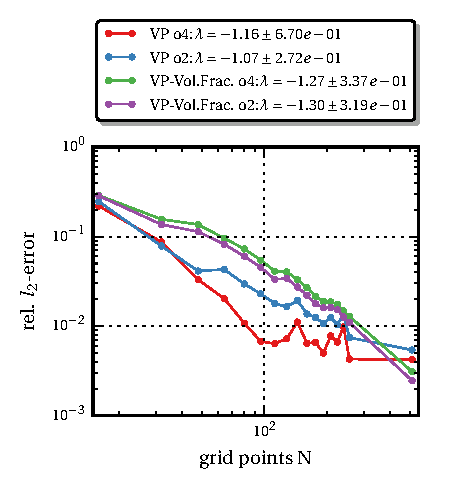
\includegraphics{gfx/immersed_boundary/tcflow/theo/vp.pdf}
      \caption{Relative $l_2$-error for different Volume-Penalization methods.}
      \label{vali:tc_flow_gc_vp}
  \end{minipage}
  \hfill
  \begin{minipage}[c]{0.45\textwidth}
      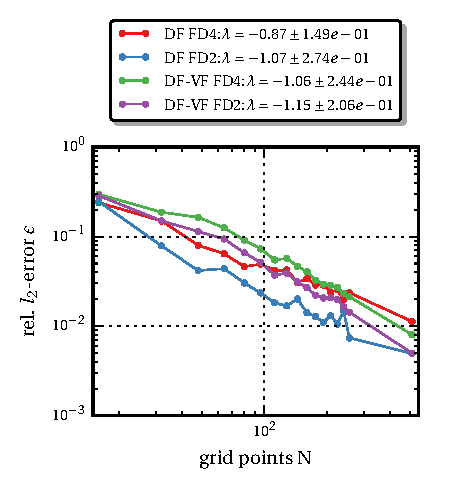
\includegraphics{gfx/immersed_boundary/tcflow/theo/df.pdf}
      \caption{Relative $l_2$-error for different Direct-Forcing methods.}
      \label{vali:tc_flow_gc_df}
  \end{minipage}

  \begin{minipage}[c]{0.45\textwidth}
      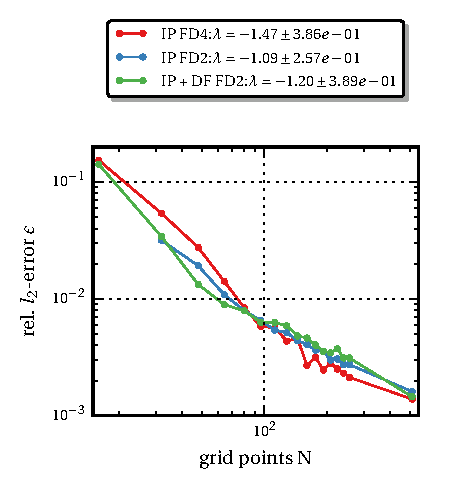
\includegraphics{gfx/immersed_boundary/tcflow/theo/ip.pdf}
      \caption{Relative $l_2$-error for different Interpolation methods.}
      \label{vali:tc_flow_gc_ip}
  \end{minipage}
  \hfill
  \begin{minipage}[c]{0.45\textwidth}
      \includegraphics{gfx/immersed_boundary/tcflow/theo/all.pdf}
      \caption{Relative $l_2$-error for the methods with the smallest error in comparison.}
      \label{vali:tc_flow_gc_all}
  \end{minipage}
\end{figure}
\clearpage

\begin{figure}[!bp]
  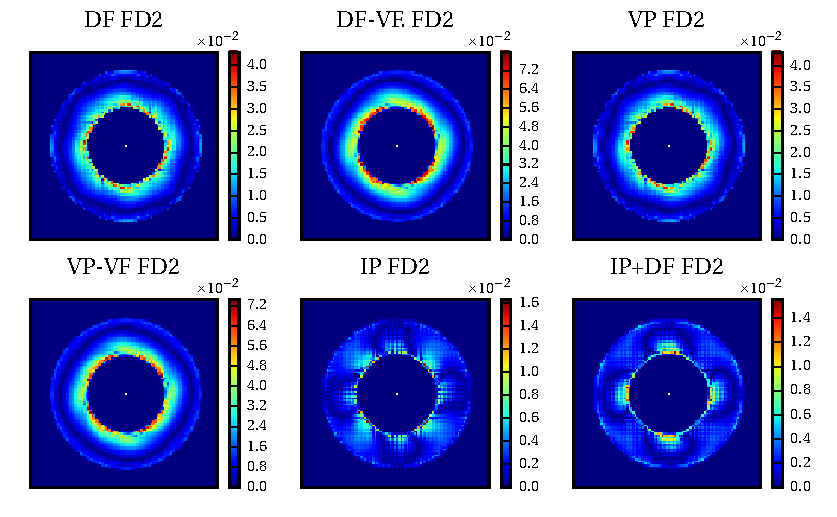
\includegraphics{gfx/immersed_boundary/tcflow/long/vz_profiles_o2.pdf}
  \caption{\label{tcflow:results_vprofiles_o2}
    Subtraction of the numerical velocity profile from the theoretical
        for all FD2 methods.}
\end{figure}

\begin{figure}[!bp]
  \begin{minipage}[c]{0.45\textwidth}
      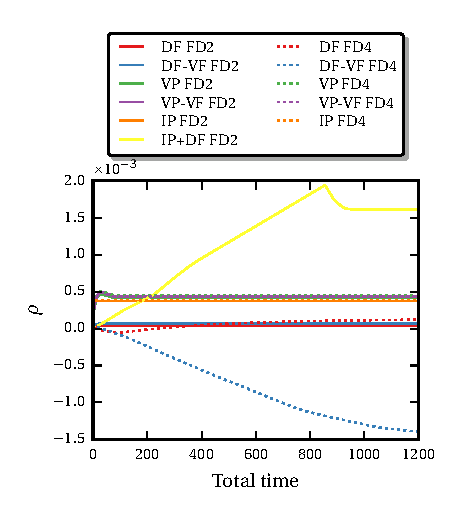
\includegraphics{gfx/immersed_boundary/tcflow/long/ts_all.pdf}
      \caption{\label{tcflow:results_long_ts_o2}
            Averaged density for FD2 methods with respect to the simulation time.
          }
  \end{minipage}
  \hfill
  \begin{minipage}[c]{0.45\textwidth}
      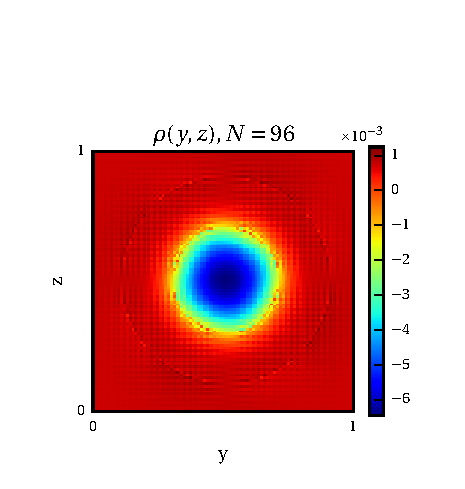
\includegraphics{gfx/immersed_boundary/tcflow/long/example.pdf}
      \caption{\label{tcflow:rho_example}
        Density oscillations for the VP-VF FD2 method with a decreased density in the inner cylinder.
      }
  \end{minipage}
\end{figure}

\clearpage

\subsubsection{Long-Term Simulations}

For all methods the simulations were numerically stable, except the IP FD4 method.
The density was averaged over the fluid domain by Eq. \ref{vali:density_calc},
the results of the computation are shown in Fig. \ref{tcflow:results_long_ts_o2}.
For the IP+DF FD2 method the density increases until a convergence is reached at $T\approx 1000$ of about $1.6\cdot10^{-3}$.
The density of the  DF-VF FD4 decreases to $-1.4\cdot10^{-3}$ with a convergence at $T\approx1400$.
For all other methods a faster convergence is reached at $T\approx200$ with an  averaged density in the order $10^{-4}$.

For all methods numerical oscillations in the density can be
observed, which  are similar to the Hagen-Poiseuille flow test case.
In Fig. \ref{tcflow:rho_example} these oscillations are exemplarily shown for the VP-VF FD2 method.
In Appendix \ref{tcflow:results_rho_profiles_o2} the remaining FD2 methods are presented.
Beside these oscillations of order $10^{-4}$ it can be noted that the density in the inner cylinder
decreases to about $-6\cdot10^{-3}$, in contrast to $\approx10^{-3}$ in the fluid domain.

\subsection{Discussion}

In this validation test case the density changes for the FD2 methods as well.
The convergence of the averaged density to the order $10^{-4}$
is similar to the previous test case with exception of the IP+DF FD2 and DF-VF FD4 method ($\approx10^{-3}$).
The decrease of the density in the inner cylinder is physical correct.
The angular velocity $\Omega_i$ creates a centrifugal force in the inner cylinder,
This results in a density distribution which is large at the outer cylinder walls and small in the center.
The negative value is not a concern since the density is undetermined by a constant.

However, it is noticeable that for the DF methods the density in the inner cylinder is zero, see Appendix \ref{tcflow:results_rho_profiles_o2}.
Since the velocities are directly set to $\vec{\Omega_i} \times \vec{r}$ in the inner cylinder,
the fluid can be considered incompressible in this domain because $\partial_t \rho = \nabla (\vec{\Omega_i} \times \vec{r}) = 0$.

The oscillations in the density can be observed for the FD2 and FD4 methods.
It can be assumed that just like in the Hagen-Poiseuille flow  an odd-even decoupling occurs.
These oscillations do not affect the numerical solutions, since
the change of velocity is proportional to $\partial \rho$ and this expression is not computed on neighboring cells.
The oscillations also occur in the FD2 methods since the density is no longer zero for these methods.%evtl rand fehler

\begin{figure}[!bp]
  \begin{minipage}[c]{0.4\textwidth}
      \centering
      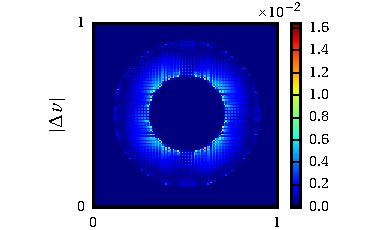
\includegraphics{gfx/immersed_boundary/tcflow/discussion/vzdiff.pdf}
  \end{minipage}
  \begin{minipage}[c]{0.6\textwidth}
      \caption{Absolute value of the velocity difference between the IP-FD2 and IP+DF-FD2 in the (x, y)-plane.
      \label{valid:hpflow_velodiff_discussion}
      }
  \end{minipage}
\end{figure}

It can be noted that the results of the IP FD2 and the IP+DF FD2 method are not equal.
This refutes the previous assumption (see Sec. \ref{sec:hpflow_discussion}),
that the velocity fields of the fluid domain and the boundaries are decoupled for FD2 methods.
Fig.\ref{valid:hpflow_velodiff_discussion} shows the subtracted velocity profiles for the IP FD2 and IP+DF FD2 method in the $(x, y)$-plane.
The largest differences between these profiles occur at the boundary of the inner cylinder, about $10^{-2}$.
Both methods create different numerical approximations at this location.
It can be noted that  the error of the IP methods is increased about one order, in comparison to the Hagen-Poiseuille flow.
For the DF and VP methods the error and convergence rates are similar.
The use of the VF method leads to an increase of the overall error, which is contrary to the Hagen-Poiseuille flow results.
The velocity difference profiles for all methods indicate a erroneous approximation of the inner boundary.
It can be assumed that the approximation of moving boundaries with Immersed Boundary methods can
lead to an overall larger numerical error.

%This is not unexpected for the VP and DF methods, since a pixelated moving boundary probably creates a to the roughness of the surface.
%From the velocity profiles it can be seen that the error of the interpolation methods is smaller at the inner boundaries.
%But still the error here is larger at the outer boundaries which indicates that moving boundaries are also difficult to interpolate with good results.


%In summary
%comparsion is much larger in compariso
%- overaall larger error and non linear decrease
%- vfrac
%- assumption inner border
%-comparison errors to the previous
%-velocity profiles indicate that the error of the methos  comes from the inner border

\clearpage

\section{Summary}

In the first part of the chapter an introduction to different Immersed Boundary methods was given.
The volume-penalization method, adapted from  \citep{Lulff2011} uses a forcing term which is proportional to the velocities at the fluid boundaries.
In case of the Direct-Forcing method, adapted from \citep{Fadlun2000} the forcing term is calculated implicitly.
Both methods were extended by the Volume-Fraction method, adapted from \citep{Fadlun2000}, which computes the fluid domain volume ratio inside a boundary
cell and uses this value as a weighting coefficient for the forcing.
Finally an interpolation method adapted from  \citep{ Gilmanov2003} was introduced. In the first step this method performs a bilinear interpolation on a surface
next to the fluid boundary, in the second step this value is linear interpolated to a grid point close to the boundary.

In the second part of the chapter three different test cases were introduced as a validation for the Immersed Boundary methods.
The laminar Poiseuille flow was used as a first validation test case for the DF and VP methods.
From the results it was possible to identify an error in the basic algorithm of the simulation.
Furthermore it could be shown that the use of a 5-Point stencil leads to discretization errors at the fluid boundaries.

In the second test case a simulation of a Hagen-Poiseuille flow was performed.
The results of this simulation pointed out possible numerical issues.
One possible problem are numerical oscillations which are assumed to be caused
by a decoupling of density field.
Furthermore this test case showed that the use of a 5-Point stencil creates a numerical error,
which results in a large error for the IP-DF4 method.
It can be noted that using the volume fraction method  the error of the DF and VP method can be improved.
In summary all errors are approximately below the order  $10^2$ for $N>100$,
by far the smallest error was obtained with the IP-DF2 method.
All convergence rates are at least as good in a comparison
to the results from validation test cases from literature.

The last test case was given by a Taylor-Couette system.
In comparison to the Hagen-Poiseuille flow the computed numerical error is larger,
up to an order for the VF methods, which perform inferior in this test case.
In this simulation for both the FD2 and FD4 methods small pressure oscillations can be observed which are again assumed to be
caused by a decoupling of the density field.
The velocity profiles show that the error is the largest to the inner domain boundary $r_i$.
This indicates that the Immersed Boundary methods in combination with implemented basic GPU algorithm
are not a good choice for moving boundaries.




